% Copyright (C)  2015 Richard Bäck.
% Permission is granted to copy, distribute and/or modify this document
% under the terms of the GNU Free Documentation License, Version 1.3 or
% any later version published by the Free Software Foundation; with no
% Invariant Sections, no Front-Cover Texts, and no Back-Cover Texts.  A
% copy of the license is included in the section entitled "GNU Free
% Documentation License".

\documentclass[a4paper,10pt]{article}
\usepackage[utf8]{inputenc} % enable umlauts in the source files
\usepackage{palatino}
\usepackage{graphicx} % use of graphics
\usepackage{amsmath} % for equotation*
\usepackage{eurosym} % the euro symbol
\usepackage{fixltx2e} % super-/subscript
\usepackage{listings} % code listings
\usepackage{fancyhdr} % headers
\usepackage{hyperref} % to create references to chapters etc.
\usepackage[version=3]{mhchem} % chemical formulas
\usepackage[german]{babel} % use german headings
\usepackage[margin=1.5cm,vmargin={0pt,1cm}]{geometry}

\DeclareGraphicsExtensions{.png}

\setlength{\headheight}{2.5cm}
\setlength{\headsep}{0.5cm}
\setlength{\textheight}{26cm}

\pagestyle{fancy}
\lhead{Richard Bäck}
\chead{}
\rhead{\today}
\lfoot{}
\cfoot{}
\rfoot{Seite \thepage}
\renewcommand{\headrulewidth}{0.4pt}
\renewcommand{\footrulewidth}{0.4pt}

\title{Zusammenschrift zu Potenzreihen}

\begin{document}
\maketitle
\thispagestyle{fancy}

\section{Taylorreihe}
\subsection{Definition}
Die Taylorreihe wird aufgestellt um eine beliebige Funktion mit einer
unendlichen Potenzreihe anzunähern. Es ist praktisch nicht möglich
eine unendliche Reihe anzulegen. Deshalb gilt: je größer n ist, desto
genauer ist die Annäherung.

\subsection{Verwendungszweck}
Eine Taylorreihe wird aufgestellt, um das Integral von einer nicht
integrierbaren Funktion zu bilden. Z.B. sind alle Funktionen, die auf
der Eulerschen Zahl aufbauen, nicht integrierbar.

\subsection{Ablauf}
\begin{enumerate}
\item { Es wird eine beliebige Funktion definiert:
    \begin{equation}
      \label{eq:1}
      f(x) := e^{-x^2}
    \end{equation}
  }
\item { Es wird eine Funktion definiert, die n-te Ableitung der
    gegebenen Funktion ermittelt:
    \begin{equation}
      \label{eq:3}
      fi(x,i) := \frac{d^i}{dx^i} \cdot f(x)
    \end{equation}
  }
\item { Es können nun mit fi() beliebig viele Ableitungen erstellt
    werden. Mit dieser können nun regelmäßigkeiten erkannt werden.
  }
\end{enumerate}

\subsection{Ablauf mit Mathcad}
\begin{enumerate}
\item { Es wird eine beliebige Funktion definiert:
    \begin{equation}
      \label{eq:1}
      f(x) := e^{-x^2}
    \end{equation}
  }
\item { Mathcad hat eine eigene Funktion integriert, die eine
    Taylorreihe mit einer Annäherung von n Summanden:
    \begin{equation}
      \label{eq:2}
      g(x, n) := f(x) Reihen, n
    \end{equation}
  }
\end{enumerate}

\section{Fourierreihe}

\subsection{Ablauf}
Gegeben soll folgende Funktion sein:\\
\begin{center}
  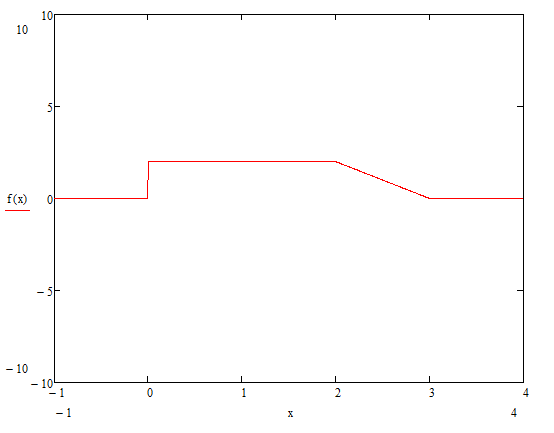
\includegraphics[height=10cm]{BeispielGraph}
\end{center}

\begin{enumerate}
\item { Nachmodellieren der gegebenen Funktion mit Hilfe von
    Entscheidungen:
    \begin{equation}
      \label{eq:5}
      \begin{split}
        f(t) := \rvert{2 if 0 \le t \le 2}\\
        \rvert{(-2 \cdot t + 6) if 2 < t \le 3}\\
        \rvert{0 otherwise}
      \end{split}
    \end{equation}
  }
\item { Festlegung der Periodenlänge:
    \begin{equation}
      \label{eq:6}
      T := 3
      \omega_0 = \frac{2 \cdot \pi}{T}
    \end{equation}
  }
\item { Berechnung der Koeffizienten:
    \begin{equation}
      \label{eq:7}
          a(n) := \frac{T}{2} \cdot \int_{0}^{T} f(t) \cdot cos(n \cdot \omega_0 \cdot t) dt
          b(n) := \frac{T}{2} \cdot \int_{0}^{T} f(t) \cdot sin(n \cdot \omega_0 \cdot t) dt
    \end{equation}
  }
\item { Modellierung der Annäherungsreihenfunktion:
    \begin{equation}
      \label{eq:8}
      fn(t,n) := \frac{a(0)}{2} + \sum_{i = 1}^{n} (a(i) \cdot cos(i \cdot \omega_0 \cdot t) + b(i) \cdot sin(i \cdot \omega_0 \cdot t))
    \end{equation}
  }
\item {
    \begin{equation}
      \label{eq:9}
      A(i) := \sqrt{a(i)^2 + b(i)^2}
    \end{equation}
  }
\end{enumerate}

\end{document}